\documentclass{etit-workshop-protokoll}

%\kursnummer{0}
%\kurstitel{Leitfaden und Vorlage zur Ausarbeitung}

%\kursnummer{1}
%\kurstitel{Messwerterfassung und regenerative Energieerzeugung}

\kursnummer{2}
\kurstitel{Analoge Filter und Schaltungsanalyse}

%\kursnummer{3}
%\kurstitel{Sensorik}

%\kursnummer{4}
%\kurstitel{Digitale Signalverarbeitung}


\gruppennummer{0}

\teilnehmer{Lukas}{Mustermann}{1245345}{utbfa}{max@example.com}
\teilnehmer{Max}{Mustermann}{1245345}{utbfa}{max@example.com}
\teilnehmer{Fabian}{Moritz}{2314434}{ufjkg}{ufjkg@kit.edu}

\begin{document}

\maketitle

\pagestyle{empty}% % leere Kopfzeile
\begin{abstract}
\section*{Zielsetzung}
Aufgabe der Arbeit ist die Entwicklung eines 2-Band-Equalizers. Dieser soll durch unabhängig Hoch- und Tiefpassfilter realisiert werden, deren Ausgänge danach in einer Addiererschaltung zusammengeführt werden. Diese Art des Zusammenführens ermöglicht eine genauere Soundeinstellung.

\end{abstract}
\clearpage % neue Seite beginnen
\pagestyle{scrheadings} % Kopfzeilen zuruecksetzen

\tableofcontents
\listoffigures
\listoftables
\clearpage % neue Seite beginnen

\section{Durchführung}
Bei der Planung eines Projekts müssen verschiedene Punkte beachtet werden, die im Folgenden einfach aufgeführt werden. Sie bilden eine solide Durchführungspraxis bei wissenschaftlichen und industriellen Projekten.
\begin{enumerate}
\item Eine Literaturrecherche wird durchgeführt, um den aktuellen Stand der Technik und der Wissenschaft zu erfahren. So kann man das eigene Projekt einschätzen und den aktuellen Stand des Projekts festlegen.
\item Projektziele müssen klar definiert werden.
\item Entwicklung von verschiedenen Lösungsansätzen und Lösungsmöglichkeiten.
\item Pro und Kontra der Lösungswege ausarbeiten.
\item Entscheidung, welcher Lösungsweg der beste scheint.
\item Erstellung eines Projektplans -- Detaillierter Arbeitsplan, der Arbeitspakete, Arbeitsabläufe, deren zeitliche Abfolge und Zwischenziele definiert.
\item Festlegung von Meilensteinen -- an welchem Punkt kann man welches Ergebnis erwarten? Es dient zur Kontrolle der Projektdurchführung.
\item Identifizierung und Analyse der einzelnen Arbeitsaufgaben.
\item Definition von Verantwortlichkeiten im Team.
\item Festlegung der Qualifikationen, die für die einzelnen Positionen im Team benötigt werden.
\item Festlegung des Budgets.
\item Besetzung der Positionen nach entsprechender Qualifikation.
\item Ausbildung neuer Arbeitskräfte für die entsprechenden Verantwortlichkeiten.
\item Entwicklung von individuellen Leistungszielen und deren Abgleich mit den entsprechenden Personen und deren Vorgesetzten.
\item Zuordnung der Aufgaben und Verantwortlichkeiten an entsprechende Personen.
\item Koordination der laufenden Projektphasen.
\item Kontrolle des Arbeitsfortschritts und Abgleich mit den Meilensteinen.
\item Kontrolle der individuellen Leistungsziele.
\item Abgleich des Arbeitsfortschritts mit den Zielen -- müssen Planänderungen vorgenommen werden?
\end{enumerate}
Viele dieser Punkte sollten Sie in Ihrem Gruppenprojekt überdenken. Sie sollten Ihr
Vorgehen im Abschlussbericht dokumentieren.
\section{Dokumentation}
Die Abschlussberichte bilden die einzige Grundlage für die Bewertung der einzelnen Kurse des Workshops. \textbf{Die Struktur Ihres Berichts sollte sich nach den Anforderungen des jeweiligen Kurses richten.}

Die folgende Struktur ist im Allgemeinen in den meisten wissenschaftlichen Schriften zu finden, wie z.\,B. in wissenschaftlichen Artikeln, Bachelor- und Masterarbeiten oder auch Dissertationen. Die Struktur kann in kleineren Dingen variieren, jedoch wird der Textkörper immer aus den folgenden Kapiteln gebildet:
\begin{itemize}
\item Abstract
\item Einleitung
\item Stand der Technik -- Literatur
\item Materialien und Methoden
\item Ergebnisse
\end{itemize}

Im Folgenden wird die Struktur des Abschlussberichts für die Projektarbeit festgelegt.
An ihr sollten sich die Abschlussberichte orientieren (eine grobe Vernachlässigung kann
zu einer negativen Bewertung führen).
\begin{itemize}
\item \textbf{Titelblatt} -- Titel der Arbeit, Autoren, Datum (Vorgegeben).
\item \textbf{Abstract} -- Kurze Zusammenfassung der Projektziele, Methoden, Ergebnisse und Diskussion (max. 1/2 DIN\,A4 Seite).
\item \textbf{Inhaltsverzeichnis} -- Kapitelübersicht. Im Allgemeinen werden nur Überschriften bis zur dritten Gliederungsebene geführt (Beispiel: Kapitel 1.1.1).
\item \textbf{Abbildungsverzeichnis} -- Liste aller Abbildungen im Bericht.
\item \textbf{Tabellenverzeichnis} -- Liste aller Tabellen im Bericht.
\item \textbf{Einleitung} -- Die Einleitung sollte einen kurzen Überblick über das Thema geben. Weiterhin sollte hier gekennzeichnet werden, wie die Projektorganisation war, welche Arbeitspakete man sich überlegt hat und wer welche Aufgaben übernommen hat.
\item \textbf{Materialien und Methoden} -- Hier sollten die verwendeten Methoden kurz beschrieben werden. Es soll kein Skript oder \glqq Lehrbuch\grqq\ sein, sondern die Methodik und Vorgehensweise zum Lösen der Ergebnisse beschreiben. D.\,h. es muss kein Kapitel über z.\,B. das Maschenstromverfahren geschrieben werden. Hier genügt ein Literaturhinweis. Oft heißt dieses Kapitel einfach \glqq Methoden\grqq. Die verwendeten Materialien sollten aber auch beschrieben werden (Beispiel: \glqq Zum Lösen des Problems wurden ein Pentium 4 mit \SI{1}{\giga B} RAM und die Software \glqq xyz\grqq\ verwendet.\grqq).
\item \textbf{Ergebnisse} -- Alle Ergebnisse sollten in diesem Kapitel präsentiert werden. Dabei muss strengstens darauf geachtet werden, dass die Ergebnisse objektiv und für jeden nachvollziehbar (alle freien Parameter spezifiziert) dargestellt werden. Alle Abbildungen müssen gut lesbar (insbesondere Achsenbeschriftungen) sein und eine erklärende Bildunterschrift haben. Beispiel: \glqq Kurve xyz zeigt ein Minimum am Punkt a\grqq\ nicht \glqq Kurve xyz erfährt durch Eigenschaft b ein Minimum am Punkt a\grqq. Letzte Aussage beinhaltet schon eine Wertung, die in dem Kapitel Diskussion behandelt werden sollte. Die Leitfrage hier sollte sein: \glqq Was kam bei der Durchführung der Methoden heraus?\grqq
\item \textbf{Diskussion} -- In diesem Kapitel werden die Ergebnisse diskutiert. Nach der objektiven Beschreibung geht es nun um Erklärungen für den Verlauf der Ergebnisse (\glqq Der Grund für das Minimum am Punkt a liegt in Eigenschaft b\grqq) und Konsequenzen aus den Ergebnissen (\glqq Aus dem Vergleich der Kurven c, d und e folgt, dass man Eigenschaft b wie in Versuch c wählen sollte\grqq).
\item \textbf{Anhang} -- Dient zu Dokumentationszwecken. Sie dürfen zusätzlich im Anhang Bilder, Diagramme oder Tabellen auch über den maximalen Umfang hinaus hinzufügen, allerdings müssen die wesentlichen Bilder, Diagramme und Tabellen innerhalb der Arbeit stehen.
\end{itemize}

Überlegen Sie sich in jeder Aufgabe und jedem Aufgabenteil, wo Sie diesen in Ihrer Dokumentation einordnen. Die einzelnen Aufgabenteile müssen also bei dieser Struktur nicht direkt untereinander eingeordnet werden. \textbf{Schreiben Sie zur Orientierung in Ihrer Dokumentation immer dazu, um welche Aufgabe es sich gerade handelt und von wem Sie bearbeitet wurde}. Aufgabenteile können auch in mehreren Kapiteln der Ausarbeitung behandelt werden. Abstract und Einleitung können keiner Aufgabe zugeordnet werden, Sie müssen diese eigenständig formulieren.

Bitte beachten Sie die Angaben über den Umfang der einzelnen Aufgabenteile falls angegeben und den maximalen Umfang der Arbeit.

Wenn Sie fremdes Gedankengut wörtlich oder sinngemäß in Ihrer Dokumentation übernehmen, muss dies durch eine Quellenangabe gekennzeichnet werden. Bei zahlreichen unterschiedlichen Quellen wird zur Erstellung eines Literaturverzeichnisses die Verwendung von Bibtex oder Biblatex empfohlen. Für wenige Quellen lässt sich das Literaturverzeichnis auch von Hand erstellen.

\subsubsection*{Gute wissenschaftliche Praxis}
\begin{itemize}
\item \textbf{Keine Textpassagen kopieren} \\
Quellen sollten nur auszugsweise wiedergegeben werden, das Kopieren ganzer Abschnitte als Literaturrecherche reicht nicht aus! Inhalte müssen selbstständig verfasst sein.
\item \textbf{Auf korrekte Quellenangaben achten} \\
Wörtlich zitierte Textpassagen sind in Anführungszeichen zu setzen (\glqq\grqq):
\begin{quote}
\glqq Mit dem Suchen von Literatur geht der Wunsch einher, die gefundenen Werke zu zitieren.\grqq\ \cite{cite}
\end{quote}
Indirekte Zitate (inhaltliche Wiedergaben) erläutern/beschreiben den Inhalt der Quelle:
\begin{quote}
Die Autoren beschreiben, dass mit der Literatursuche der Wunsch einhergeht, gefundene Werke zu zitieren \cite{cite}.
\end{quote}
Quelle entsprechend im Literaturverzeichnis aufführen:
% Achtung, dies ist nicht die korrekte Weg, ein Literaturverzeichnis in LaTeX einzufuegen. Fuer den korrekten Weg orientieren Sie sich am Inhalt der Datei 'literatur.tex'.
\begin{quote}
\begin{tabularx}{\textwidth}{>{\hsize=.02\hsize}X>{\hsize=.8\hsize}X}
[1] & \url{http://www.starkerstart.uni-frankfurt.de/43759138/FB09-Musikwissenschaften-Richtiges-Zitieren.pdf}, Abrufdatum: 30. November 2016.
\end{tabularx}
\end{quote}
\end{itemize}
\section{Abgabe der Projektarbeit}
Als Prüfungsleistung muss ein Bericht abgegeben werden. Zur Erstellung des Berichts wird die Nutzung dieser \LaTeX-Vorlage empfohlen, da dort bereits alle Einstellungen für die Formatierung gesetzt sind und der Umgang mit \LaTeX\ damit gut trainiert werden kann. Wenn Sie den Bericht mit einem Textverarbeitungsprogramm erstellen, verwenden Sie 12 Punkt Schriftgröße und \num{1,5}-fachen Zeilenabstand. Stellen Sie die Marginalien auf \SI{2,5}{\centi \meter} rechts und links, oben \SI{2,5}{\centi \meter} und unten \SI{2}{\centi \meter}.

Es muss klar erkenntlich sein, wie die Projektarbeit organisiert und durchgeführt wurde. Aus dem Bericht muss klar hervor gehen, wer welchen Teil bearbeitet hat und wer welchen Teil der Arbeit geschrieben hat (z.\,B. eine Tabelle in die Einleitung, wer welchen Teil bearbeitet hat oder den Autor des Kapitels an den Anfang des Kapitels stellen). Die Ergebnisse müssen eindeutig sein, insbesondere welches Projektmitglied welche Aufgaben übernommen hat und welche Teile gemeinsam bearbeitet wurden.

Der fertige Bericht muss bis zum Abgabeschluss als pdf-Datei in Ilias hochgeladen werden. Bitte beachten Sie, dass jeder Teilnehmer der Gruppe aus technischen Gründen den Bericht einzeln hochladen muss. Bis zum Abgabeschluss kann die Berichtsversion auf Ilias aktualisiert werden, es wird nur die letzte Version gewertet. Die Bewertung der Aufgabe kann nach Korrektur in Ilias eingesehen werden.
\section{Leitpunkte der Bewertung}
Die folgenden Punkte werden bei der Bewertung der Aufgabe besonders berücksichtigt:

\subsubsection*{Form:}
\begin{itemize}
\item Struktur des Berichts
\item Erscheinungsbild
\item Klar erkennbare Projektorganisation
\end{itemize}

\subsubsection*{Vollständigkeit:}
\begin{itemize}
\item Bearbeitung der Aufgaben
\end{itemize}

\subsubsection*{Ergebnisse:}
\begin{itemize}
\item Qualität
\item Diskussion
\item Schlussfolgerungen
\end{itemize}
\section{Vorlage}
Sie können dieses Dokument unmittelbar als Vorlage für die Erstellung Ihrer Dokumentation verwenden. Die Klassen-Datei \verb|etit-workshop-protokoll.cls| legt dabei das Format fest und sollte daher nicht verändert werden.

Das Dokument wird durch die Hauptdatei \verb|etit-workshop-protokoll-bsp.tex| erzeugt. Dort können Sie den jeweiligen Kurs auswählen, indem Sie die entsprechenden Zeilen ein- und auskommentieren. Nutzen Sie anschließend die vorgegebenen Befehle um Ihre Gruppe und die einzelnen Gruppenmitglieder auf der Titelseite anzugeben.

In der Hauptdatei folgt dann der eigentliche Inhalt des Dokuments. Zunächst wird die Titelseite erstellt, die Sie unverändert übernehmen können. Anschließend wird das Abstract eingebunden, gefolgt von den Verzeichnissen. Die jeweiligen Abschnitt sind zur besseren Übersichtlichkeit in einzelnen Dateien verfasst, die mit \verb|\include{}| oder \verb|\input{}| in das Dokument eingefügt werden. 

Für Ihre Dokumentation können Sie die einzelnen Quelldateien austauschen oder deren Inhalt beliebig anpassen. Die folgenden Beispiele können Ihnen beim Schreiben helfen. Schauen Sie sich bei Unklarheiten auch den Quellcode dieses Dokuments an, um nachzuvollziehen, wie die einzelnen Inhalte dieses Abschnitts erzeugt wurden.

\subsection{Gleichungen}
\begin{align}
    \int_{-\infty}^{\infty}\exp{-x^2}\;\mathrm{d}x &= \sqrt{\pi}\\
    \int_0^{\infty}\frac{x}{e^x-1}\;\mathrm{d}x&=\frac{\pi^2}{6}
\end{align}


\subsection{Einheiten}
Für Einheiten steht das Paket \verb|siunitx| zu Verfügung. Dadurch werden Einheiten in der richtigen Schriftart (aufrecht) gesetzt.
\begin{verbatim}
    \SI{1}{\micro m\per s} = \SI{3,6e-6}{\km\per h}
\end{verbatim}
\begin{align}
    \SI{1}{\micro m\per s} = \SI{3,6e-6}{\km\per h}
\end{align}


\subsection{Abbildungen}
Abbildungen werden mit dem Befehl \verb|\includegraphics{dateiname}| eingebunden. Die Dateiendung muss dabei nicht explizit angegeben werden. Mit \verb|pdflatex| können direkt \textit{.jpg}, \textit{.png}, \textit{.bmp} oder \textit{.pdf} Dateien eingefügt werden. %Wenn \verb|latex| mit \verb|dvips| und \verb|ps2pdf| verwendet wird, müssen .eps-Dateien eingebunden werden.
\begin{verbatim}
\begin{figure}[htb]
    \centering
    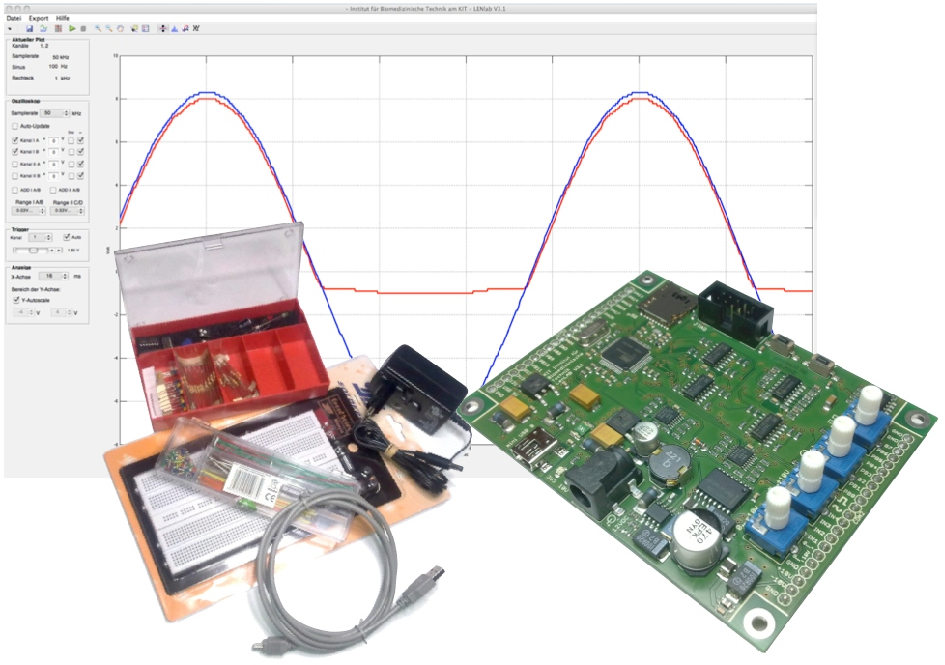
\includegraphics[width=8cm]{etit_titelbild}
    \caption{Die Materialien der Projektarbeit.}
    \label{fig:materialien}
\end{figure}
\end{verbatim}

Mit dem \verb|\ref|-Befehl lässt sich im Fließtext auf Abbildungen verweisen, z. B. verweist \verb|\ref{fig:materialien}| auf die Workshopmaterialen in Abbildung \ref{fig:materialien}, wo zuvor mit dem \verb|\label|-Befehl die Kennung \verb|fig:materialien| definiert wurde.

\begin{figure}[htb]
    \centering
    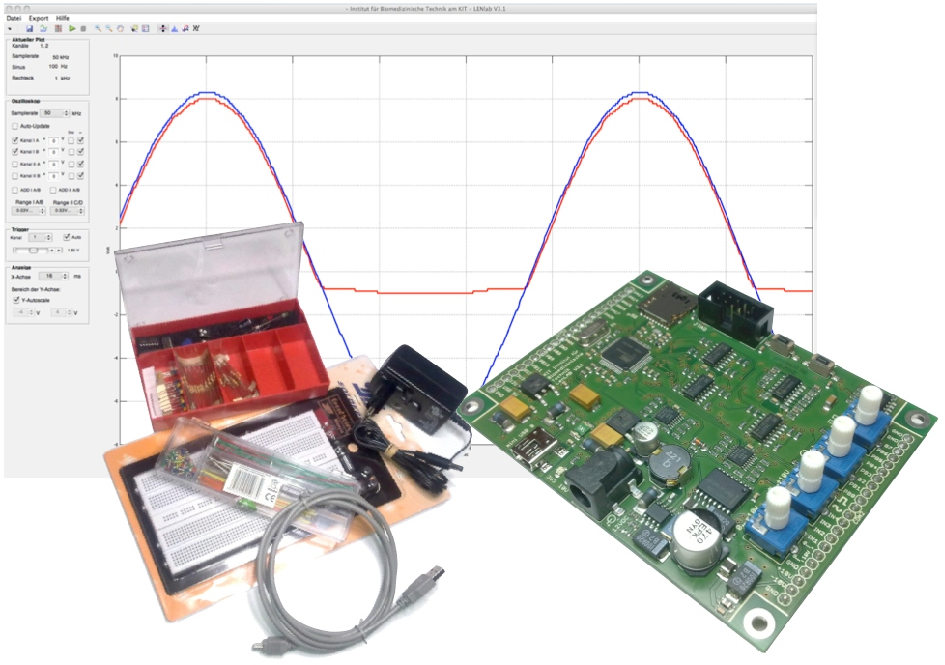
\includegraphics[width=8cm]{etit_titelbild}
    \caption{Die Materialien der Projektarbeit.}
    \label{fig:materialien}
\end{figure}


\subsection{Tabellen}
Eine beispielhafte Messreihe ist in Tabelle \ref{tab:messwerte} angegeben.
\begin{table}[htb]
    \centering
    \caption{Messwerte Widerstand.}
    \label{tab:messwerte}
    \begin{tabular}{ccc}
        \toprule
        Spannung [\si{\volt}] & Strom [\si{\ampere}] & Widerstand [\si{\ohm}] \\
        \midrule
        \num{10} & \num{5} & \num{2} \\
        \num{20} & \num{2} & \num{10} \\
        \bottomrule
    \end{tabular}
    
\end{table}


\subsection{Aufzählungen}
Aufzählungen werden mit der \verb|itemize|-Umgebung erzeugt.
\begin{itemize}
    \item Erster Punkt.
    \item Zweiter Punkt.
\end{itemize}


\subsection{Literatur}
Im Text wird mit dem \verb|cite|-Befehl auf Buchquellen \cite{bronstein}, Konferenzbeiträge \cite{kalman} und Internetquellen \cite{atmel} verwiesen. Auf jede Referenz im Literaturverzeichnis muss mindestens einmal im Text verwiesen werden.


\subsection{Quelltext}

Mit der \verb|lstlisting|-Umgebung kann MATLAB-Quelltext direkt in der \LaTeX-Datei eingegeben werden.

\begin{verbatim}
\begin{lstlisting}[style=matlab]
% Matlab-Logo
A = membrane; 
figure 
surf(A); 
colormap('cool');
\end{lstlisting}
\end{verbatim}

\begin{lstlisting}[style=matlab]
% Matlab-Logo
A = membrane; 
figure 
surf(A); 
colormap('cool');
\end{lstlisting}

Ein komplettes MATLAB-Skript kann mit dem Befehl
\begin{verbatim}
\lstinputlisting[style=matlab]{Beispiel.m}
\end{verbatim}
eingebunden werden. Ersetzen Sie einfach den Dateinamen \textit{Beispiel.m} durch Pfad und Namen Ihres Skripts. Die Ausgabe des Skripts stellt sich wie folgt dar.
\lstinputlisting[style=matlab,caption={Beispiel-Matlab-Code.}]{Beispiel.m}

Das kleine MATLAB-Programm \textit{Beispiel.m} zeigt außerdem die Verwendung des Befehls \textit{latex.m}. Fügen Sie dazu die Datei \textit{latex.m} in das MATLAB-Verzeichnis ein bzw. stellen Sie über \textit{Set Path} sicher, dass MATLAB den Ordner, in dem sich die Datei befindet, kennt. Mit \verb|latex(M)| können Sie dann die Matrix $M$ im Befehlsfenster von MATLAB in der Form ausgeben lassen, dass Sie sie direkt in Ihr \LaTeX-File kopieren können, wie folgendes Beispiel zeigt.
\begin{verbatim}
\begin{table}[htb]
\centering
\caption{Tabelle erzeugt mit Beispiel.m}
\label{Beispieltabelle}
\begin{tabular}{ccc}
\toprule
Zeit & $\sin$-Funktion & $\cos$-Funktion\\
\midrule

$0.00000$ & $0.00000$ & $1.0000$ \\
$1.0000$ & $0.84147$ & $0.54030$ \\
$2.0000$ & $0.90930$ & $-0.41615$ \\
$3.0000$ & $0.14112$ & $-0.98999$ \\
$4.0000$ & $-0.75680$ & $-0.65364$ \\
$5.0000$ & $-0.95892$ & $0.28366$ \\
$6.0000$ & $-0.27942$ & $0.96017$ \\

\bottomrule
\end{tabular}
\end{table}
\end{verbatim}
Die gezeigte Sequenz erzeugt dann Tabelle \ref{tab:Beispieltabelle}.
\begin{table}[htb]
    \centering
    \caption{Tabelle erzeugt mit Beispiel.m.}
    \label{tab:Beispieltabelle}
    \begin{tabular}{ccc}
        \toprule
        Zeit & $\sin$-Funktion & $\cos$-Funktion\\
        \midrule
        $0.00000$ & $0.00000$ & $1.0000$ \\
        $1.0000$ & $0.84147$ & $0.54030$ \\
        $2.0000$ & $0.90930$ & $-0.41615$ \\
        $3.0000$ & $0.14112$ & $-0.98999$ \\
        $4.0000$ & $-0.75680$ & $-0.65364$ \\
        $5.0000$ & $-0.95892$ & $0.28366$ \\
        $6.0000$ & $-0.27942$ & $0.96017$ \\
        \bottomrule
    \end{tabular}
\end{table}

Quelltext in anderen Formaten, z. B. \LaTeX- oder C-Code, kann ebenfalls mit dem Befehl \verb|\lstinputlisting| eingebunden werden.

\clearpage % neue Seite beginnen
\begin{thebibliography}{99}
\bibitem{cite} \url{http://www.starkerstart.uni-frankfurt.de/43759138/FB09-Musikwissenschaften-Richtiges-Zitieren.pdf}, Abrufdatum: 30. November 2016.
\bibitem{atmel} Atmel Corporation. 32-bit ATMEL AVR Microcontroller AT32UC3B0256. \url{http://www.atmel.com/devices/at32uc3b0256.aspx}, Abrufdatum: 15. Oktober 2013.
\bibitem{bronstein} I. N. Bron\v{s}tejn, K. A. Semendjajew, G. Musiol und H. Mühlig (Hrsg.). {\itshape Taschenbuch der Mathematik}. Verlag Harri Deutsch, Frankfurt am Main, 8. Auflage, 2012.
\bibitem{kalman} R. E. Kalman. A New Approach to Linear Filtering and Prediction Problems. In: {\itshape Transactions of the ASME--Journal of Basic Engineering}, Bd. 82 (D), S. 35--45, 1960.
\end{thebibliography}

\end{document}

